\documentclass[12pt]{article}

\hbadness=10000
\hfuzz=50pt
\pdfminorversion=9

\usepackage{graphicx}
\usepackage{subfig}
\usepackage{url}
\usepackage{algorithm}
\usepackage{algorithmic}
\usepackage{listings}
\usepackage{amsmath}
\usepackage{amsthm}
\usepackage{verbatim}

\usepackage{booktabs}
\usepackage{colortbl}
\usepackage{tabularx}
\usepackage{color}
\usepackage{xspace}
\usepackage{hyperref}    % Creates hyperlinks from ref/cite 
\hypersetup{pdfstartview=FitH}

%\graphicspath{{../figures/psware/}{../figures/shm/}{../simulation/psware/}{./figures/}{./simulation/}{../Percom2011/simulation/}{../Percom2011/figures/}}
\graphicspath{{./simulation/}{../figures/psware/}{../simulation/psware/}}

\newcommand{\HRule}{\rule{\linewidth}{0.5mm}}
\newcommand{\figurecurrentwidth}{\includegraphics[width=\textwidth]}
\newcommand{\figurehalfwidth}{\includegraphics[width=.5\textwidth]}
%\newcommand{\figurecurrentwidth}{\includegraphics[width=.49\textwidth]}
%\newcommand{\figurehalfwidth}{\includegraphics[width=.24\textwidth]}
\lstset{float, numbers=left, frame=lines, belowcaptionskip=3mm, xleftmargin=7mm, framexleftmargin=7mm, escapeinside={(*}{*)}, tabsize=3, breaklines=true}
\newtheorem{theorem}{Theorem}

\renewcommand{\algorithmicrequire}{\textbf{Input:}}
\renewcommand{\algorithmicensure}{\textbf{Output:}} 
\floatname{algorithm}{Procedure}

\begin{document}

\title{PSWare: A Flexible Middleware Framework for Composite Event in Wireless Sensor Network}
\author{
{Scribus Primus}\\
\affaddr{Primus Address}\\
\email{primus@somewhere.com} \and
{Scribus Secundus}\\
\affaddr{Secundus Address}\\
\email{secondus@elsewhere.com}
}
\conferenceinfo{SenSys'11,} {November 1--4, 2011, Seattle, WA, USA.}
\CopyrightYear{2011}
\crdata{XXX-X-XXXXX-XXX-X}
\maketitle
\begin{abstract}
Event detection is an important topic in many WSN applications. Although there are several works on providing event-based services in WSN, most of them can only deal with primitive event types but cannot handle composite events very well. In general, a type-based event system may have primitive or composite event types. All event types are defined by specifying their attributes and filters. Then, individual events are detected and delivered according to such type information. Composite event types may be defined by combining multiple event types with operators. Due to the resource constraints in WSN, composite events are much more difficult to manage than primitive events. In this work, we introduce PSWare, a type-based publish / subscribe middleware for WSN that supports composite events. We describe our design for PSWare. PSWare has a flexible architecture where different composite event detection algorithms may be easily integrated.

On top of PSWare, we present TED (Type-based Event Detection), a novel distributed composite event detection algorithm. The essential idea of TED is event fusion, where some sensor nodes are selected as fusion points and component events are fused for the detection of a high level event. Event fusion with minimum energy cost is an NP-complete problem. Therefore, TED uses a number of heuristics with bounded performance.  

To further increase the performance of event detection, we design a clustering algorithm for PSWare for structural health monitoring applications (SHM). We formulate the problem and found it to be NP-complete so we propose heuristic centralized and distributed algorithms. In addition to SHM, We use PSWare to develop other real world WSN applications including intelligent transportation system (ITS) and in-door monitoring.

We evaluate our system from different aspects. We first evaluate TED, the most essential algorithm in our system. We analyze its performance and then carry out extensive simulations. Both analytical and simulation results show TED can save energy in event-based applications where primitive events occur in a higher frequency than composite events. Then we combine TED with PSWare and carried out some real world experiments. The results show that PSWare can offer reasonably simple API for the application developers to use while TED and our clustering algorithm can improve the underlying event detection performance. Compared with opportunistic approaches to event detection in these real applications, PSWare can reduce 40 - 50 \% of the energy cost.
\end{abstract}

\chapter{Introduction}
\section{Overview}
\label{sec:introduction}
Development in wireless communication and electronics has made it possible to create low-cost, low-power wireless sensor nodes. Each sensor node usually contains a wireless transceiver, a micro processing unit and a number of sensors. The sensor nodes can collect data and do some simple processing locally, and can communicate with each other to form an ad hoc wireless sensor network (WSN) \cite{aky:survey}. A WSN is usually self-organized and self-maintained without any human intervention. Wireless sensor networks have been used in various application areas such as smart building \cite{lynch:shm}, wild environment monitoring \cite{wsnhabitat}, intelligent transportation systems \cite{klein:its}, battle surveillance \cite{wsntracking} and healthcare \cite{lo:ban}. 

While WSN has a wide range of applications, programming sensor networks is a challenging because different from programming in the traditional environment. WSN imposes a lot of constraints such as limited computational power, less memory and unreliable communication. Application developers need to not only understand the requirements for the specific application domain but also take into consideration of the characteristics of WSN. In this research work, we propose PSWare, a publish/subscribe (pub/sub) middleware for WSN which eases the development of WSN applications. Our middleware uses a pub/sub programming paradigm for the application programmer to subscribe application specific events. It provides an easy-to-use Event Definition Language (EDL) to allow the application developers to define composite events while uses a flexible architecture so that different domain-specific event processing algorithms can be easily integrated into the middleware.

\subsection{Motivation}
Despite the large variety of WSN applications, many of them are essentially event-based. In applications such as intelligent transportation systems \cite{klein:its}, smart buildings \cite{lynch:shm} and healthcare \cite{lo:ban}, the events sensor nodes detect events which reflect the environmental changes and the systems respond to these events accordingly. Events may be primitive or composite. Primitive events (e.g. when the temperature exceeds certain threshold) can be detected by a single sensor node without having to cooperate with others. On the other hand, \emph{composite events} consist of multiple primitive events. They reflect a serial of environmental changes with spatial and temporal relations among them and must be detected collaboratively by different sensor nodes.

Because of the common requirements and challenges for composite event subscription and detection, it is more desirable to have a generic middleware layer to handle composite events instead of reinventing the wheel and implementing application-specific event processing mechanisms. In addition, the middleware should be flexible enough so that different event processing algorithms for different application domains can be easily integrated. In summary, the middleware should achieve the following design goals:
\begin{enumerate}
\item \emph{Event abstraction}: since composite events are collaboratively processed by different sensor nodes in the network, they introduce extra complexity because of the resource constraints and unreliable communication. A middleware framework providing high level event abstraction is needed to ease the application development.
\item \emph{Re-usability and flexibility}: different applications may share certain common modules during event processing. They may also have other different modules. A middleware framework can help so that common modules may be used and different modules may be replaced without affecting others.
\end{enumerate}

\subsection{Issues}
In this research, we address the essential issues of designing and developing PSWare. On the highest level, an event description language is provided to allow users to describe composite event relationships. On the lowest level, a runtime environment is necessary on each sensor nodes so that they could understand and execute the event processing algorithms translated from the high-level EDL. More specifically, we need to address the following research/engineering issues to make our middleware work.

\begin{itemize}
\item	\emph{Event definition language}: we need to provide an event description language which is powerful yet easy to use.
\item	\emph{Event definition language compiler}: a compiler is essential to translate the programs written in our high-level language into a low-level language understandable by the sensor nodes. The compiler must be smart enough to extract the semantic meanings from the program and do some optimization.
\item	\emph{Runtime environment support}: the middleware running on each sensor node should provide a runtime environment to execute the compiled programs.
\item	\emph{Subscription propagation}: after the program written in EDL is compiled, the subscription should be intelligently disseminated into the network. If the subscription is too big, it may need to be divided into small ones. Furthermore, only related sensor nodes need to be updated.
\item	\emph{Event detection}: we need to design efficient protocol for the sensor nodes to cooperate with each other to detect composite events.
\item	\emph{Event delivery}: after the subscribed the events have been detected, we need energy-efficient routing protocols so that the detected events will be delivered at the minimum cost.
\end{itemize}
\section{Background}
\label{sec:background}
\begin{comment}
We first briefly overview the issues in event subscription and event detection.
\end{comment}
\subsection{Event Types and Subscriptions}
Each event contains a list of attributes which are the actual data obtained from the sensors. Users can subscribe events with subscriptions which specify event types and event filters. Different event types can have relations among each other. The relations may also be expressed as special type of filters that operate on multiple event types. Listing \ref{prog:compositeExample} shows how a composite event type is defined \cite{lai:psware}. The event type 'CompTemp' requires two sub-events of type 'AvgTemp'. The two sub-events must satisfy certain temporal constraints in order to indicate the occurrence of the composite event.
\begin{lstlisting}[caption=Example of a composite event, label=prog:compositeExample]
Event CompTemp {
} on {
    AvgTemp e1 and
    AvgTemp e2
} where {
    e2.time-e1.time=600
}
\end{lstlisting}
\begin{comment}
Mathematically, event types together with their relations can be represented by a directed acyclic graph, where each node represents an event and each edge represents a relation. The nodes with 0 indegree represent primitive event types which are the events that can be directly obtained from individual sensor nodes. The rest of the nodes represent composite event types. The event type which has 0 outdegree is the subscribed event type.
\end{comment}
Once the subscriptions are defined, it will be disseminated into the network so that sensor nodes start to detect the corresponding events. In a pub/sub system, if an event is detected to match the subscribed event type, it will be delivered to the sink to notify the subscriber.

\subsection{Type-based Event Detection}
In our approach to event detection, we make use of some special nodes called event fusion points. These nodes take the responsibility of composite event detection. The event fusion points may have some extra capabilities in terms of processing power or storage though it's not compulsory. For each event fusion point, it has an event detection framework as shown in Figure \ref{fig:eventdetectionframework2}. In such a framework, events are stored in a buffer and associated with types. Each event type has a corresponding filter so that the fusion points can decide if the event occurs or not. The event filters consist of some predicates on the event attributes.
Event detection based on our model involves three steps:
\begin{enumerate}
\item Detect an event either locally or receive an event from other nodes. Then store it in the buffer. 
\item Look up for the corresponding filter for that event.
\item Evaluate the event against the filter.
\item If the event is evaluated to have happened, make a decision on where to send the event.
\end{enumerate}

\begin{figure}
\centering
\figurecurrentwidth{eventdetectionframework2}
\caption{Type-based event detection framework}
\label{fig:eventdetectionframework2}
\end{figure}

The event detection framework in Figure \ref{fig:eventdetectionframework2} is essentially type-based event detection because the predicates are grouped according to the event types. In addition, compared with topic or content-based approach, type-based event detection is more suitable for WSN-based applications. Because of the resource constraints in WSNs, it is usually not efficient to send all the primitive events to the sink node for centralized event detection. Instead, events should be detected in-network if possible. Composite events in WSNs may have multiple levels and higher level events cannot be detected until its sub-events have been detected. Therefore, in-network event detection must take the event types into consideration in order to detect the events.  

\begin{comment}
Second, pure topic based event detection may not be suitable for WSNs because many WSNs require events that have different data types or topics. For example the detection of fire may require both temperature and light event topics. Without considering event types, it is very difficult to do in-network composite events detection just based on the event topics. Third, similar to topic based event detection, content based event detection without considering event types can only filter the primitive events and may not be efficient if the lower-level events occur with a much higher frequency than composite events.
\end{comment}
\section{PSWare: Model and Architecture}
\label{sec:model}
In this section, we describe the application programming model for PSWare. We keep the issues that described in Section \ref{sec:introduction} when establishing our model.

\subsection{Overview}
\begin{figure}
\centering
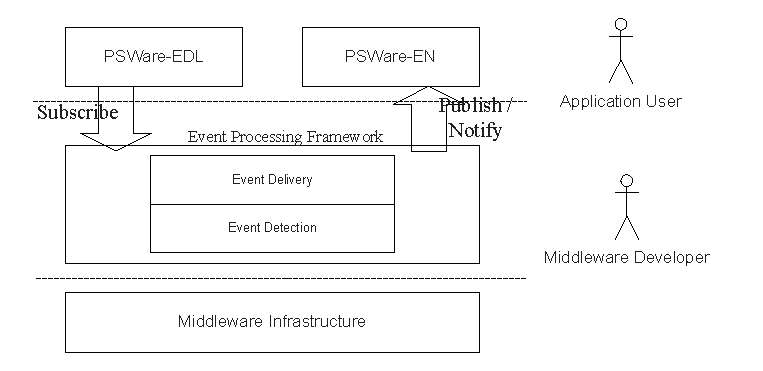
\includegraphics[width=\textwidth]{programmingModel}
\caption{PSWare programming model}
\label{fig:programmingModel}
\end{figure}

As shown in figure \ref{fig:programmingModel}, our model mainly has two different types of people that make use of two APIs of different levels:
\begin{itemize}
\item Application developers will make use of the event definition language to define and subscribe events and use the event receiving module to receive the published events.
\item Middleware developer will make use of the event processing framework to implement effective and efficient event processing algorithms
\end{itemize}

The first type is the application users. These users are responsible for defining and subscribing to high level events for different types of applications. They use a high level event definition language to translate the application requirements into events. They do not have to worry about the underlying event detection mechanisms.

On the lower level, we have another type of users called middleware developers. These users are responsible for implementing domain-specific event processing mechanisms. PSWare provides a couple of interfaces in TinyOS to make the implementation easier.

The benefit for such model is its flexibility. There are usually many different types of applications for a specific application domain. For example, in ITS, we may have collision warning, traffic flow control and overspeed detection yet these applications can probably share a lot of common event detection mechanisms. Therefore, the middleware developer only needs to implement the event processing mechanism for once. Then by defining different events, we can easily meet different application requirements without sacrificing the efficiency.

\subsection{Event Definition Language}
\begin{figure}
\centering
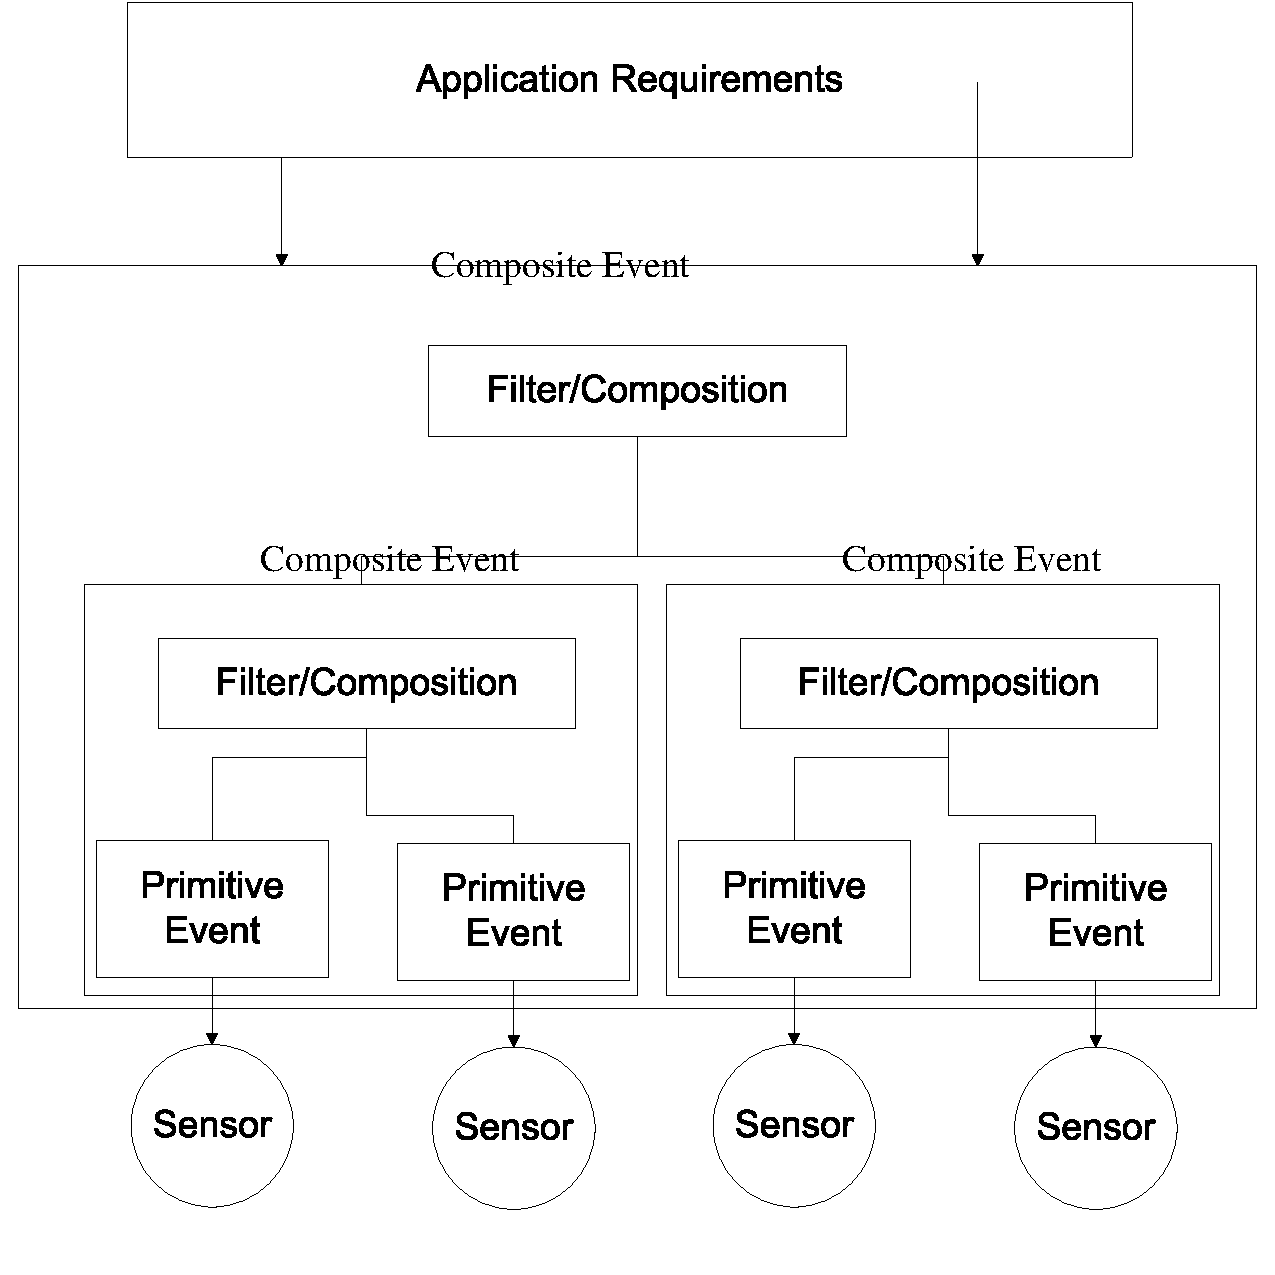
\includegraphics[width=.6\textwidth]{eventprogramming}
\caption{Type-based event model}
\label{fig:eventprogramming}
\end{figure}

PSWare will provide an type-based event programming model to the application user. Such model has the following characteristics:
\begin{itemize}
\item Each event type is similar to a class in object-based programming model. Similarly, event hierarchy in Figure \ref{fig:eventhierarchy} is similar to class hierarchy.
\item Similar to object-based model, attributes are encapsulated in each events.
\item Event definition are declarative. The high-level application developers only need to specify the event filters and event relations through operators and functions. The underlying mechanisms for implementing these operators are left to our event detection framework.
\end{itemize}

Figure \ref{fig:eventprogramming} conceptually shows our event model. On the top level, the application requirements are expressed in terms of the composite events that need to be detected. The composite events may be further divided into sub-events. Eventually all composite events can be divided into primitive events which can be directly detected by individual sensor nodes.

To re-use our example in Section \ref{sec:introduction}, Figure \ref{fig:rooms}, we may define the events as shown in Listing \ref{lst:rooms}.
\begin{lstlisting}[caption=Example of using even-based programming model, label=lst:rooms]
Event SimpleEvent {
	int temp=System.temp;
	int id=System.id;
	int time=System.time;
} where {
	temp > 30
}
Event CompEvent {
} on {
	SimpleEvent e1 and
	SimpleEvent e2
} where {
	e1.Location="A" and
	e2.Location="B" and
	e2.time-e1.time=600
}
\end{lstlisting}

We can see that our event-based programming model shares some of the similarity with SQL, especially for the event filters, which consist of operators. In this particular example, we have two event types. On the top level, the application wants to monitor the temperature change so the event type 'CompEvent' is defined. 'CompEvent' consists of two sub-events of the same type: SimpleEvent. Note that our programming model is declarative. The user just specifies the event types and the corresponding filters without specifying the event detection strategies described in Section \ref{sec:introduction} because that part is left to the event detection framework. We will go into more details in that in the latter part of this section.

\subsection{Event Notifier}
Apart from submitting event definition, the application user needs to be notified when the subscribed events are detected by WSN. This is done through event notifier. When the application user subscribes events, the user needs to pass an additional object as the event notifier. When the subscribed event is detected, PSWare will notify the user with this notifier object. Listing \ref{lst:notiferJava} shows our notifier class implemented and how it is related to the subscription class.

\begin{lstlisting}[caption=Event notifier in Java, label=lst:notiferJava]
public interface EventNotifier {
	public void notify(String eventStr);
	...
}
public class EventSubscription {
	public Boolean subscribe(String subscription, EventNotifier notifier) {
		...
	}
}
\end{lstlisting}

While Listing \ref{lst:notiferJava} shows the notifier in Java, bindings for other languages can be created in similar fashion. A Python binding is shown in Listing \ref{lst:notiferPython}.
\begin{lstlisting}[caption=Python binding of event notifier, label=lst:notiferPython]
class EventNotifier:
	def notify(self, eventStr):
		pass
class EventSubscription:
	def subscribe(self, subscription, notifier):
		...
\end{lstlisting}

Upon the detection of events, the notifier will be invoked so that the events can be delivered to the user. The event is delivered as a string, with each attribute assigned with an actual value. As an example, suppose the user has subscribed to the event 'SimpleEvent' in Listing \ref{lst:rooms}, then when the event is detected by PSWare, it will be delivered to the user with the content shown in Listing \ref{lst:eventFormat}.
\begin{lstlisting}[caption=Received event from notifier, label=lst:eventFormat]
SimpleEvent e1 {
	temp=32;
	id=0;
	time=13345;
}
\end{lstlisting}

\subsection{API for Event Processing Framework}
The event processing framework of PSWare is developed using NesC. PSWare also provides a group of APIs for the middleware developers to write customized event processing algorithms. First, since all events can ultimately be decomposed into primitive events, the middleware developer needs to first define the required primitive events used in the application domain. This is done through a configuration named 'PrimitiveEventC'. It is listed in Listing \ref{lst:primitiveEvent}. The new event ID should be defined as an enumeration in PSWare's header file.
\begin{lstlisting}[caption=Primitive event component in NesC, label=lst:primitiveEvent]
generic configuration PrimitiveEventC(evet_id_t eventId) {
  provides {
    interface Read<uint16_t>;
  }
} implementation {
	...
}
\end{lstlisting}

In PSWare, everything is treated as events and that includes temperature, photo and even timer. Similar to other generic components in TinyOS, if necessary, new events can be added by implementing a new event ID. Once set, we need to create a higher level primitive event so that the application users can make new event definitions based on top of it. This is done by an automatic tool which will be invoked when building and output a class which will be used by the event notifier and an event definition which will be used by EDL.

When this is set, the application user can already start to subscribe and detect events by using PSWare's default event detection algorithm: TED \cite{lai:ted}. If the middleware developer wants to write their own event detection algorithm, they can choose to implement two interface 'EventMatcher' and 'EventDeliver' as shown in Listing \ref{lst:pswareEventMatcher}. The 'EventMatcher' interface includes two major event which serves three purposes as follows:
\begin{enumerate}
\item During the execution of the middleware, the network may detect multiple events for a single event type. Therefore, upon the detection of the composite events, the event detection algorithm may choose a specific event from one of this sub-types for detection. This is done by signaling the first event 'select sub-event'.
\item Upon the detection of an event, the event detection algorithm may perform some customized processing to update some information so that the next time when the event happens again, it may be detected with lower cost. This is when the second event 'eventMatched' comes into play. The middleware developer may implement customized event processing mechanisms according to the matched events.
\end{enumerate}

Apart from event matcher, we also have an event deliverer which will be called when a subscribed event is detected. The middleware developer may implement its only function to meet the requirements for event delivery. This is done when the middleware signals the 'eventDeliver' event.
\begin{lstlisting}[caption=The event matcher interface, label=lst:pswareEventMatcher]
interface EventMatcher {
	event bool selectSubevent(EventInstanceInfo * composite, EventInstanceInfo * subevent);
	event result_t eventMatched(evet_id_t eventId, evet_id_t instanceID, bool detectionResult);
}
interface EventDeliverer {
	event result_t eventDeliver(evet_id_t eventId, evet_id_t instanceID, bool detectionResult);
}
\end{lstlisting}

To facilitate the implementation of event matcher and event deliverer, the middleware developer can make use of the APIs provided by PSWare in Listing \ref{lst:pswareAPI}. These APIs are mostly used to retrieve the event information.
\begin{lstlisting}[caption=PSWare API in NesC, label=lst:pswareAPI]
interface EventType {
	command EventTypeInfo * getEventType(evet_id_t eventId);
	command bool isSubscribed(evet_id_t eventId);
	command bool isComposite(evet_id_t eventId);
}
interface EventInstance {
	command int instanceAmount(evet_id_t eventId);
	command EventInstanceInfo * getEventInstance(evet_id_t eventId, evet_id_t idx);
	command void deleteEvent(evet_id_t eventId, evet_id_t instanceID);
}

typedef struct {
	evet_id_t eventId;
	evet_id_t level;
	size_t size;
} EventTypeInfo;

typedef struct {
	evet_id_t typeID; (*\label{lst:pswareAPI:typeID}*)
	evet_id_t instanceID;
	uint16_t * attributes;
} EventInstanceInfo;
\end{lstlisting}

The first interface, 'EventType' has three commands. The first command is for the individual event instances to obtain the type information based on their type ID as shown on line \ref{lst:pswareAPI:typeID}. The second and the last commands are self-explanatory. They are used to determine if a given event type is a composite event or is subscribed by the user.

Since for each event type, there can be multiple events, we need the second interface 'EventInstance' to process those events. There are three commands for this interface. The first one is used to obtain the number of the events for a specific type currently stored in the event buffer on the sensor node. We will discuss about the event buffer in the next section. Upon knowing the number of events, the middleware developer can iterate through the event list and use the second command to get the events. As for the last command, when an event is detected to be useless, the middleware developer may delete it from the list.

The data structures are shown after the interfaces. For event type, we have the ID for the type, its level in the subscribed event tree and its size. For the event instance data structure, we have its type ID, instance ID and its attribute list. If the event contains some attributes of the primitive events, they can be obtained here by using the index defined in the enumeration value for primitive event. For instance, if one of the primitive event has an enumeration value labeled 'EVENT\_LIGHT', then if the event instance also has one of its attribute from the sensor's light reading, the middleware developer can access it by writing 'attributes[EVENT\_LIGHT]'.

In summary, the middleware developer may follow the following steps to implement customized event detection algorithms:
\begin{itemize} 
\item Implement new primitive event types if necessary.
\item Define the event matcher for how sub-events are selected for matching and what to do after a predefined event type is detected.
\item Define customized function for event delivery.
\end{itemize}
\begin{figure}
\centering
\figurecurrentwidth{psware-architecture}
\caption{Event processing in PSWare}
\label{fig:psware-architecture}
\end{figure}

\section{Composite Event Processing in PSWare}
\label{sec:design}
In this section, we discuss how PSWare is designed to support composite event. The overall work flow of event processing in PSWare is shown in Figure \ref{fig:psware-architecture}. To use the middleware, applications developers will first define event types according to the application requirements. The subscription will then be compiled and processed by the EDL compiler and be disseminated into the network. When the events are detected by the sensor nodes, they will be delivered to the application.

\subsection{Event Specification}
\begin{figure}
\centering
\figurecurrentwidth{edlcompiler}
\caption{PSWare-EDL compiler structure}
\label{fig:edlcompiler}
\end{figure}

EDL is used for specifying events in PSWare. For each EDL script, it contains one or more event definition and one subscribing statement. Formally, the BNF of the subscription is defined in Listing \ref{lst:BNFSubscription}.

\begin{lstlisting}[caption=BNF (simplified) of subscription, label=lst:BNFSubscription]
subscription -> event_declarations subscribe_statement
event_declarations -> event_declaration | event_declarations event_declaration
subscribe_statement -> SUBSCRIBE IDENTIFIER SEMICOLON
\end{lstlisting}

The subscribe statement simply uses the keyword 'subscribe' followed the event type name needed by the application. Each event type declaration can have up to three parts: the event body, the where clause and the on clause. The event body defines the attributes of the events. The on clause are used to specify the sub-events used by a composite event. The where clause defines the filter of the corresponding event type. Formally, the BNF of event type is defined in Listing \ref{lst:BNFEvent}

\begin{lstlisting}[caption=BNF (simplified) of event type, label=lst:BNFEvent]
event_declaration -> EVENT IDENTIFIER event_body on_clause_opt where_clause_opt
event_body -> { field_declarations_opt }
on_clause -> ON { subevent_declarations_opt }
where_clause -> WHERE { conditional_expression }
\end{lstlisting}

The on clause and the where clause are both optional in case if the event is primitive or does not have a filter. The on clause looks similar to the field declaration except sub-events instead of fields are declared. This is done for a clear code presentation and easier type checking. The where clause simply consists of conditional expressions so that the filters may be defined by specifying the operators.

\begin{comment}
A simple example of using EDL is shown in Listing \ref{lst:originaledl}. In this example, two events, 'SimpleEvent' and 'CompEvent' are defined. 'SimpleEvent' is a primitive event which occurs when the detected temperature reading is above certain threshold. 'CompEvent' is a composite event that is based on two events of 'SimpleEvent' and their time must satisfy a certain condition in order to indicate the occurrence of 'CompEvent'.
\begin{lstlisting}[caption=A simple EDL program, label=lst:originaledl]
Event SimpleEvent {
	int temp=System.temp;
	int id=System.id;
	int time=System.time;
} where {
	temp > 30
}
Event CompEvent {
} on {
	SimpleEvent e1 and
	SimpleEvent e2
} where {
	e2.time-e1.time=600
}
\end{lstlisting}
\end{comment}

The EDL-based subscription will be processed by our EDL compiler. The output of the compiler has two parts as shown in Figure \ref{fig:edlcompiler}. The first part is the byte codes which will be executed by individual sensors to detect events. The format and the organization of the byte codes are closely related to the event processing framework and customization of PSWare. We will go through these topics in the following sections.

\begin{figure}
\centering
\figurecurrentwidth{edlcompiler-flow}
\caption{EDL compiler flow}
\label{fig:edlcompiler-flow}
\end{figure}

The second part, the event receiving module is the implementation of the event notifier as discussed in Section \ref{sec:model}. As shown in Figure \ref{fig:edlcompiler-flow}, The EDL compiler will execute the following steps in order to generate the byte codes and event receiving module:
\begin{enumerate}
\item Parse the EDL script and generate the corresponding syntax tree and symbol table.
\item Generate the byte codes based on the syntax tree and symbol table.
\item Create the event receiving module based on the symbol table.
\end{enumerate}

\subsection{Runtime Environment for Event Detection}
The byte codes generated by the compiler can be further divided into three parts: event meta data, event filters and event matcher. These components implements the programming interface discussed in Listing \ref{lst:pswareAPI} and \ref{lst:pswareEventMatcher}. Event meta data contains the description of the event types such as event type ID, event size and the individual attributes for each event. Event filters are the constraints defined for each event type. Event matcher schedules the execution for event detection according to the subscription and event relations.

The runtime environment on each sensor node is similar to the VM-based approach \cite{mate} in the sense that the subscriptions are broken down into some basic operations called instructions. Such design choice is for extensibility so that new features can be added more easily by adding new instructions. In addition to the VM-based runtime environment, each sensor node has an event buffer where the detected events can be stored for composite event detection.

\begin{figure}
\centering
\figurecurrentwidth{eventdetectionframework2}
\caption{PSWare runtime environment}
\label{fig:eventdetectionframework2}
\end{figure}
The essential operations for our runtime environment is shown in Figure \ref{fig:eventdetectionframework2}. In this environment, the event matcher will first fetch the events from the event buffer and then evaluate them against the corresponding filters. If the event has been detected, then it will be transmitted over the network. Formally, the procedure of the event matcher can be shown in Procedure \ref{algo:eventmatcher} with some notations defined as:
\begin{itemize}
\item Event types: \(E=\{e_1, e_2 \cdots \}\)
\item For each \(e_n\in E\), its filter is: \(e_n\rightarrow filter\)
\item For each \(e_n\in E\), it has a set of events \(E_n=\{e_n^1, e_n^2 \cdots \}\) stored in the buffer.
\end{itemize}

\begin{algorithm}
\begin{algorithmic}
\REQUIRE \(E\)
	\FORALL {\(e_n\in E\)}
		\FORALL {\(e_n^i\in E_n\)}
			\IF {\(e_n\) is primitive}
				\STATE result = evaluate\_primitive (\(e_n^i\))
				\IF {result == True}
					\STATE eventMatched(\(e_n^i\))
					\IF {\(e_n\) is subscribed}
						\STATE deliver(\(e_n^i\))
					\ELSE
						\STATE forward(\(e_n^i\))
					\ENDIF
				\ENDIF
			\ELSE
				\STATE \(e_{sub} = \emptyset \)
				\FORALL {subevents \(e_m\) for \(e_n\)}
					\STATE \(e_{sub} = e_{sub}\bigcup selectSubevent (e_n, e_m)\)
				\ENDFOR
				\FORALL {subevents \(e_m\) for \(e_{sub}\)}
					\STATE evaluate\_composite(\(e_n^i\), \(e_m\), \(\cdots \))
				\ENDFOR
			\ENDIF
		\ENDFOR
	\ENDFOR
\end{algorithmic}
\caption{Procedure of the event matcher}
\label{algo:eventmatcher}
\end{algorithm}

There are several keys in the procedure. First, when the event matcher picks up the events of type \(e_n\) from the event buffer, it may use application specific mechanisms to pick up the desired events instead of trying all the possible combinations. Second, the 'deliver()' and the 'forward()' function are used to deliver the subscribed events or forward the events so that composite events may be detected. These two functions may also be application dependent to achieve high energy efficiency.

\begin{comment}
Figure \ref{fig:psware-interaction-simple} illustrates how different components in the middleware system interact with each other.

\begin{figure}
\centering
\figurecurrentwidth{psware-interaction-simple}
\caption{PSWare-E components interaction}
\label{fig:psware-interaction-simple}
\end{figure}
\subsection{PSWare Customization}
\end{comment}

Finally, it is necessary to mention the 'SystemEvent'. This module acts as the device driver for PSWare. It defines the sampling rate and a primitive event. All the fields of other events are obtained from 'System'. The module needs to implement three interfaces: StdControl, SystemClock and SystemEvent as shown in Listing \ref{lst:systemEvent}. StdControl is a module for initialization purpose. SystemClock defines the sampling frequency. SystemEvent is used to obtain the pointer to the 'System' event.

\begin{lstlisting}[caption=API of the 'System' event, label=lst:systemEvent]
module SystemEventM {
	provides {
		interface StdControl;
		interface SystemEvent;
		interface SystemClock;
	}
}
interface SystemEvent {
	command EventInstanceInfo * get();
}
\end{lstlisting}

The 'SystemEvent' is there so that needs to be implemented by the middleware developers as the  Once the 'System' event is defined, the application developers can further define their own functions for event delivery and event forwarding. We will show some examples in the next section. 
\section{Flexibility in PSWare}
In this section, we discuss how PSWare can achieve the desired flexibility in different aspects of an event-based system, namely, event detection, event delivery and event subscription.

\subsection{Flexibility in Event Detection}
Event detection is the heart of an event-based system. However, different applications may have very different requirements on event detection. For example, many WSN-applications may want to minimize energy consumption to extend network life span. Fortunately, in PSWare, we can easily customize the event detection algorithm by using the middleware framework.

We demonstrate the flexibility in event detection through two examples in this subsection. The first example is TED \cite{lai:ted} which is an event detection algorithm that aims at minimizing energy consumption. The second example is 

The essential idea of TED is fusion point selection, where the sensor nodes detect events and select parent nodes according to the detection cost so that the cost for future event detection can be reduced.

%Need to use a new figure
\begin{figure}
\centering
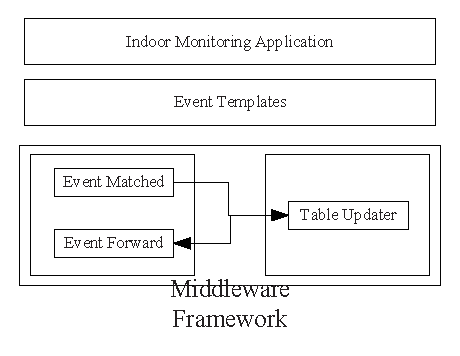
\includegraphics[width=.8\textwidth]{indoor-architecture}
\caption{TED over PSWare}
\label{fig:ted-architecture}
\end{figure}

\begin{algorithm}
\begin{algorithmic}
\REQUIRE \(v_n\rightarrow msg_r\)
	\FOR {each entry \(t'\) in \(msg_r\)}
		\IF {\NOT exists \(t'\rightarrow fid_n\) in \(table_r\)}
			\STATE \(addTo(table_r, t')\)
		\ENDIF
		\FOR {each entry \(t\) in \(table_r\)}
			\IF {\(t\rightarrow fid_n = t'\rightarrow f_n\)}
				\IF {\(t'\rightarrow hop_n < t\rightarrow hop_n\)}
					\STATE \(t\rightarrow hop_n \gets t\rightarrow hop_n+1\)
					\STATE \(t\rightarrow parent_n \gets v_n\)
				\ENDIF
			\ENDIF
		\ENDFOR
	\ENDFOR
	\IF {self is fusion point \AND \NOT exists \(self\rightarrow id\) in \(table_r\)}
		\STATE \(addTo(table_r, (self\rightarrow id, 0, self\rightarrow id))\)
	\ENDIF
	\STATE \(msg_r \gets table_r\)
	\STATE \(periodically\_broadcast(msg_r)\)
\end{algorithmic}
\caption{\(table_r\) construction}
\label{algo:table_r}
\end{algorithm}

In TED, we have a set of nodes \(V'\subseteq V\) selected as event fusion points. Each individual sensor nodes will maintain the following table \(table_r\) for all \(v'_n\in V'\)
\begin{itemize}
\item Fusion point ID (\(fid_n\)): the node ID of the fusion point:
\item	Hop count (\(hop_n\)): the number of hops to reach the fusion point
\item	Parent (\(parent_n\)): the next hop to that fusion point\\
\end{itemize}
Each sensor node will also maintain an event table \(table_e\) containing the information for each event type \(e_n\in E\) which includes the following fields:
\begin{itemize}
\item Event type ID (\(e_n\)): the ID which is assigned to each event type
\item Fusion point for the event (\(fusion_n\)): the fusion point at which the event is mostly likely to be detected at the lowest cost.
\item Fusion cost (\(cost_n\)): the fusion cost for event type \(e_n\)\\
\end{itemize}
In addition to the above tables, each fusion point \(v'\in V'\) will maintain another table \(table_m\) for the purpose of matching events. \(table_m\) contains the following fields:
\begin{itemize}
\item Event type ID (\(e_n\)): the ID of the event type
\item Event instance ID (\(i\)): the \(i\)th event instance of event type \(e_n\) (we use \(e_n^i\) to denote such an instance of event)
\item Source node (\(v_n^i\)): the node which forwarded \(e_n^i\) to the fusion point
\item Event timestamp (\(t_n^i\)): the timestamp when the event \(e_n^i\) is detected
\item Detection cost (\(cost_n^i\)): the cost for detecting event \(e_n^i\)
\end{itemize}

Each node \(v_n\) periodically broadcasts messages \(msg_r\) which is its \(table_r\). If the node itself is a fusion point, then it will add itself in \(table_r\) and broadcast the message. The procedure is shown in Procedure \ref{algo:table_r}.

In addition to \(msg_r\), each \(v'_k\in V'\) will periodically advertise its \(table_m\) by broadcasting \(msg_m\) so that other sensor nodes can construct their \(table_e\) with Procedure \ref{algo:table_e}.

\begin{algorithm}
\begin{algorithmic}
\REQUIRE \(v'_k\rightarrow msg_m\)
	\FOR {each entry \(t'\) in \(msg_m\)}
		\IF {\NOT exists \(t'\rightarrow e_n\) in \(table_e\)}
			\STATE \(addTo(table_e, (t'\rightarrow e_n, 1, v'_k, t'\rightarrow cost_n^i+table_r\rightarrow hop_k))\)
		\ENDIF
		\FOR {each entry \(t\) in \(table_e\)}
			\IF {\(t\rightarrow e_n = t'\rightarrow e_n\)}
				\IF {\(t'\rightarrow cost_n^i+table_r\rightarrow hop_k < t\rightarrow cost_n\)}
					\STATE \(t\rightarrow cost_n \gets t'\rightarrow cost_n^i+table_r\rightarrow hop_k\)
					\STATE \(t\rightarrow fusion_n \gets v'_k\)
				\ENDIF
			\ENDIF
		\ENDFOR
	\ENDFOR
	\IF {self is fusion point}
		\STATE \(msg_m \gets table_m\)
		\STATE \(periodically\_broadcast(msg_m)\)
	\ENDIF
\end{algorithmic}
\caption{\(table_e\) construction}
\label{algo:table_e}
\end{algorithm}

The construction of \(table_m\) will take place when the event instance \(e_n^i\) is detected and forwarded to a fusion point \(v'_n\). We will discuss how forwarding could be done in the next subsection.

When an event \(e_n^i\) is detected at node \(v_k\), node will use \(table_r\) and \(table_e\) to decide how to forward the detected event to the fusion points so that higher level events can be detected. The pseudo code is shown in Procedure \ref{algo:eventforwarding}.

\begin{algorithm}
\begin{algorithmic}
\REQUIRE detected event \(e_n^i\)
	\IF {\(table_e\rightarrow fusion_n=null\)}
		\STATE \(event\_forward(e_n^i)\)
	\ELSE
		\STATE \(send(e_n^i, table_e\rightarrow fusion_n)\)
	\ENDIF
\end{algorithmic}
\caption{Event forwarding}
\label{algo:eventforwarding}
\end{algorithm}

In case the fusion point for event type \(e_n\) has not been decided, the node will forward the event to some of its closet fusion points using the \(event\_forward\) function according to TED. Upon the reception of \(e_n^i\) from \(v_k\), the fusion point will first update its own \(table_m\). Then it will check if there is any composite event \(e_{comp}\) which uses \(e_n\) and another event \(e_j\) as its sub-event (\(e_{comp}=comp(e_n, e_j)\)). The pseudo code of event matching is shown in Procedure \ref{algo:eventmatching}.

\begin{algorithm}
\begin{algorithmic}
\REQUIRE \(e_n^i\) detected by \(v_k\) with cost: \(cost_n^i\)
	\STATE \(addTo(table_m, (e_n, e_n^i, v_k, now(), cost_n^i))\)
	\FOR {each \(e_j\) in \(E\)}
		\IF {\(\exists r\in R\) \AND \(r=e_{comp}=comp(e_n, e_j)\)}
			\FOR {each \(e_j^k\) in \(table_m\)}
				\IF {\(comp(e_n^i, e_j^k)=true\)}
					\STATE \(addTo(table_m, (e_{comp}, e_{comp}^i, self, now(), cost_n^i+cost_j^k))\)
					\STATE \(detected(e_{comp})\)
				\ENDIF
			\ENDFOR
		\ENDIF
	\ENDFOR
	\STATE \(event\_forward(e_n^i)\)
\end{algorithmic}
\caption{Event matching}
\label{algo:eventmatching}
\end{algorithm}

Note that if \(e_{comp}\) has been successfully detected, the procedure will run function \(detected\) which, in turn, will execute Procedure \ref{algo:eventforwarding}. The procedure will also use \(event\_forward\) in the end to forward the detected event to other fusion node so that better fusion point may be found.

Next 
\subsection{Flexibility in Event Delivery}

\subsection{Flexibility in Event Subscription}
\section{Application Scenarios}
\label{sec:pswareImpl}
In previous sections, we have introduced PSWare and how it can be customized to meet different application requirements. In this section, we demonstrate how PSWare can help in developing practical WNS applications through three application case studies: the indoor monitoring, the car park and the intelligent transportation system.

The key features of the three applications are as follows:
\begin{itemize}
\item Energy efficiency in an indoor monitoring system is crucial because the network needs to operate for a long period of time and it is not necessary to gather all the raw data.
\item Reliability is important in a car park system because the management system needs to know the time when each car enters and leaves the car park so as to calculate the fee.
\item Event detection and delivery mechanism may be tailor-made for an ITS system because transportation network has certain special 
\end{itemize}

\subsection{Applications Overview}
Indoor environment monitoring uses WSN for monitoring because it is easy to deploy the sensor nodes. Such application domain has many applications including air-conditioning, fire alarm and office space light adjustment. Such system is a good application for using composite events because of the following characteristics:
\begin{itemize}
\item There may be a large amount of raw data since the data may be gathered from a lot of sources.
\item The users may not be interested in all the raw data. Instead, they may be more interested in change of the data. This is because the events such as fire or temperature change will usually trigger the change of the sensory data. 
\item Primitive event detection may not be sufficient. For instance, a fire alarm may be characterized by a combination of different types of events such as temperature and light.
\end{itemize}

In the area of intelligent transportation system (ITS), WSN also finds many applications because it is easy to deploy the sensor nodes without interrupting the traffic. This application also has a lot of applications including collision avoidance, traffic light control, automatic road enforcement and electronic toll. Composite event detection is very common in these applications because one of the common requirements for these applications is to detect the speed of vehicle. However, different from the indoor temperature and light monitoring, the ITS applications have the following characteristics:
\begin{itemize}
\item The magnetic sensor used in ITS application will consume much more energy so the energy consumption from sensing may not be negligible. This will affect the event detection method for ITS.
\item The sensor nodes are deployed and lined up on each road and will detect each passing vehicle one by one. Such special deployment may also affect the event detection method.
\item Events may need to be delivered to mobile sinks instead of a fixed point.
\item Different types of events may require different event delivery methods. Urgent events such as accident may need to be disseminated in a real time fashion while events such as road condition and weather information may be delivered in a delay tolerant fashion.
\end{itemize}

Intelligent car park systems is an application domain which is related to ITS. However, it is different from other ITS applications in the following ways:
\begin{itemize}
\item The detected events usually need to be delivered to a central management center instead of to mobile vehicles.
\item The deployment of the sensor nodes is different. In a car park system, it is usually not necessary to deploy the sensor nodes on the roads. Instead, they are usually deployed in individual parking space to keep track of availability of them.
\item Different from other ITS applications, the event delay in intelligent car park is not as important. Message delay for a couple of seconds is probably acceptable.
\end{itemize}

On the other hand, a car park system is also different from our first indoor application in the sense that:
\begin{itemize}
\item Each message must be reliably delivered so that the management system can correctly record the entrance and exit time and calculate the parking fee.
\item The environment for message transmission may be harsh because cars are usually made of metal. Therefore, message lost may be common.
\end{itemize}
To meet the reliability requirement, we need to implement special event detection and delivery mechanisms so that the events can be reliably detected and delivered in such an unreliable environment.

\subsection{Discussion}
The requirements for the indoor monitoring application can be met with TED since the primary goal of TED is to reduce energy consumption by filtering the events which will not lead to the detection of subscribed composite events. To have a practical application scenario, we deployed our sensor nodes around the Internet and Mobile Computing Laboratory of the Hong Kong Polytechnic University. The deployment plan is shown in Figure \ref{fig:indoorDeployment}.

\begin{figure}
\centering
\figurecurrentwidth{indoorDeployment}
\caption{Deployment of the senosr nodes for indoor monitoring}
\label{fig:indoorDeployment}
\end{figure}

We use this deployment for two applications: fire detection and temperature control. Since it is infeasible to transmit all the raw data to the sink, some nodes in the network will have be used as local decision maker and detect the composite event. As a result, developing the application will involve the following steps:
\begin{enumerate}
\item Deploy the network and select the appropriate sensor nodes as event fusion points using the fusion point selection algorithm in TED.
\item Subscribe the desired events through PSWare.
\item Detect the composite events with PSWare.
\item Automatically let the nodes switch between different event fusion points to achieve high efficiency.
\end{enumerate}

To monitor the temperature change of the entire floor and adjust the air-conditioner accordingly, we need to define a composite event that comprises of the sub-events for individual room. For example, the air conditioner can be adjusted if several adjacent rooms' temperature rises too fast. The primitive and composite event definitions for this purpose are shown in Listing \ref{prog:indoorEvents}.

\begin{lstlisting}[caption=Event definition for temperature monitoring, label=prog:indoorEvents]
Event SingleTemp {
	int id=System.id;
	int temperature=System.temperature;
} where {
	temperature>THRESHOLD
}
Event CompositeTemp {
} on {
	SingleTemp e1, e2, e3;
} where {
	e1.id==1 &&
	e2.id==2 &&
	abs(e1.time - e2.time)<TIME_INTERVAL
}
\end{lstlisting}

The primitive event simply tests if the temperature passes certain threshold while the composite event is the conjunction of several primitive events. We deployed the some Micaz nodes in different rooms in our building as shown in Figure \ref{fig:indoorDeployment}.

For fire alarm, the composite event definition is based on both light and temperature readings. The event definition is shown in Listing \ref{prog:indoorFire}.
\begin{lstlisting}[caption=Event definition for fire alarm, label=prog:indoorFire]
Event Temperature {
	int id=System.id;
	int temperature=System.temperature;
} where {
	temperature>THRESHOLD_TEMP
}
Event Light {
	int id=System.id;
	int light=System.light;
} where {
	light>THRESHOLD_LIGHT
}
Event Fire {
} on {
	Temperature temp;
	Light light;
} where {
	e1.id==light.id
}
\end{lstlisting}

\begin{figure}
\centering
\subfloat[Road side sensor nodes]{\label{fig:itsSensor1}\figurehalfwidth{itsSensor1}}
\subfloat[Sensor nodes on the lamp]{\label{fig:itsSensor2}\figurehalfwidth{itsSensor2}}
\caption{Sensor nodes for transportation systems}
\label{fig:itsSensor}
\end{figure}

While TED works fine for indoor applications, it is not suitable for ITS. Because its unique characteristics as described in the previous subsection, we need to implement different event detection algorithm so as to improve its efficiency. Because of the high energy cost of sensing, the sensor nodes will turn their sensors off for most of the time while keeping their radio on so that they can know when to start sensing. Furthermore, sensor nodes are deployed along the roads and events are also forwarded along the roads so that . The procedure for nodes' wake-up and forwarding is shown in Procedure \ref{algo:itsForward}. We use the following notations in the procedure:
\begin{itemize}
\item \(V=\{v_1, v_2 \cdots \}\): the sensor nodes that come next on the road. For the sensors on the road, \(\|V\|=1\) but for the sensors next to the crossroads, \(\|V\|>1\)
\item Vehicle events \(e_i\) which are either detected locally or received from another node.
\end{itemize}

\begin{algorithm}
\begin{algorithmic}
	\IF {detected vehicle event \(e_i\)}
		\FORALL {\(v_n\in V\)}
			\STATE forward \(e_i\) to \(v_n\)
		\ENDFOR
	\ENDIF
	\IF {received vehicle event \(e_i\) from \(v_m\)}
		\STATE start data collection
		\IF {detected vehicle event \(e_j\)}
			\STATE select \(e_i\) and \(e_j\) for composite event detection
		\ELSE
			\STATE wait for event to expire
		\ENDIF
		\STATE stop data collection
	\ENDIF
\end{algorithmic}
\caption{Event forwarding for ITS}
\label{algo:itsForward}
\end{algorithm}

In the actual application deployment as illustrated in Figure \ref{fig:itsSensor}, we use some sentry nodes at the entrances of the deployed area. These nodes have more power and will monitor the entrance for newly entered cars. Except for the sentry node, the nodes will not actively collect data until it receives messages from others. Once the event from the previous node on the road is received, it will be selected for composite event detection.

As for the event definition in ITS applications, we will illustrate one of the basic events used in such applications: the tracking for vehicles. The event definition is shown in Listing \ref{lst:carEvent}.

\begin{lstlisting}[caption=Event definition for tracking vehicles, label=lst:carEvent]
Event CarEvent {
	int time=System.time;
	int magnetic=System.magnetic;
	int location=System.location;
} where {
	magnetic>THRESHOLD
}
Event SpeedEvent { (* \label{lst:carEvent:speed} *)
	int speed=(e1.location-e2.location)/(e1.time-e2.time);
} on {
	CarEvent e1, e2;
} where {
	e1.time>e2.time &&
	speed>THRESHOLD
}
\end{lstlisting}

First, an event named 'CarEvent' is defined to detect the presence of the individual vehicles. Then based on this event, we can define a composite event to measure the speed of the car as on Line \ref{lst:carEvent:speed}.

\begin{figure}
\centering
\subfloat[The sensor node]{\label{fig:carParkSensor1}\figurehalfwidth{carParkSensor1}}
\subfloat[The light sensor]{\label{fig:carParkSensor2}\figurehalfwidth{carParkSensor2}}
\caption{Car park sensor platform}
\label{fig:carParkSensor}
\end{figure}

We used the campus car park as our test bed for intelligent car park system applications. We deployed some micaz sensor nodes for the application. For simplicity, we use light sensor to detect the presence of a vehicle. For better communication, the sensor nodes are attached close to the ceiling instead of on the ground. The light sensor on each node is connected through an extended cable as shown in Figure \ref{fig:carParkSensor}. 

\begin{figure}
\centering
\figurecurrentwidth{carParkDeployment}
\caption{Car park sensor deployment}
\label{fig:carParkDeployment}
\end{figure}

The deployment of the individual sensor nodes is shown in Figure \ref{fig:carParkDeployment}. In such a system, the management is interested in the number of park spaces and the location of them \cite{tang:carpark}. Therefore, each parking space is monitored by one sensor node.
The primitive events for such a system will be the availability of individual car park spaces. Based on the primitive event, if we want to get notified when the parking spaces near the exit become available, then we just need to define composite events which locate the spaces with certain IDs. Th event definitions are shown in Listing \ref{prog:carPark}. Here, the composite event takes two primitive events for parking space \(1\) and \(2\) which are close to the exit.

\begin{lstlisting}[caption=Event definition for a car park, label=prog:carPark]
Event ParkSpaceEvent {
	int id=System.id;
	int time=System.time;
	int light=System.light;
} where {
	light>THRESHOLD
}
Event CarParkEvent {
	int id=System.id;
} on {
	ParkSpaceEvent e1, e2;
} where {
	e1.id==1 ||
	e2.id==2 ||
	e1.time-e2.time<10
}\end{lstlisting}
%\section{Application Scenarios}
\label{sec:pswareImpl}
In previous sections, we have introduced PSWare and how it can be customized to meet different application requirements. In this section, we demonstrate how PSWare can help in developing practical WNS applications through three application case studies: the indoor monitoring, the car park and the intelligent transportation system.

The key features of the three applications are as follows:
\begin{itemize}
\item Energy efficiency in an indoor monitoring system is crucial because the network needs to operate for a long period of time and it is not necessary to gather all the raw data.
\item Reliability is important in a car park system because the management system needs to know the time when each car enters and leaves the car park so as to calculate the fee.
\item Event detection and delivery mechanism may be tailor-made for an ITS system.
\end{itemize}

\subsection{Application Overview}
An indoor monitoring system can have many different purposes including air-conditioning, fire alarm and office space light adjustment. Such system is a good application for using composite events because of the following characteristics:
\begin{itemize}
\item There may be a large amount of raw data since the data may be gathered from a lot of sources.
\item The users may not be interested in all the raw data. Instead, they may be more interested in change of the data. This is because the events such as fire or temperature change will usually trigger the change of the sensory data. 
\item Primitive event detection may not be sufficient. For instance, a fire alarm may be characterized by a combination of different types of events such as temperature and light.
\end{itemize}

To have a practical application scenario, we deployed our sensor nodes around the Internet and Mobile Computing Laboratory of the Hong Kong Polytechnic University. The deployment plan is shown in Figure \ref{fig:indoorDeployment}.

\begin{figure}
\centering
\figurecurrentwidth{indoorDeployment}
\caption{Deployment of the senosr nodes for indoor monitoring}
\label{fig:indoorDeployment}
\end{figure}

We use this deployment for two applications: fire detection and temperature control. Since it is infeasible to transmit all the raw data to the sink, some nodes in the network will have be used as local decision maker and detect the composite event. As a result, developing the application will involve the following steps:
\begin{enumerate}
\item Deploy the network and select the appropriate sensor nodes as event detectors. We borrow the idea from TED \cite{lai:ted} and call these event detectors event fusion points. In our deployment, we select the nodes 14, 16 and 0 as fusion points.
\item Subscribe the desired events through PSWare.
\item Detect the composite events with PSWare.
\item Automatically let the nodes switch between different event fusion points to achieve high efficiency.
\end{enumerate}

\subsection{Overall Architecture}
Based on our requirement analysis, we have the system architecture shown in Figure \ref{fig:indoor-architecture}. On the bottom layer, we have PSWare as well as a module for selecting event fusion points. During the event detection process, the fusion point selection will be executed in parallel and the sensor nodes will switch between fusion points to minimize the detection cost. The two modules interact with each other mainly through two interfaces: when an event is matched, the fusion selection module will be called to update the some tables so that when the event is detected again later, the module can be called again to select the better node for forwarding the event.

\begin{figure}
\centering
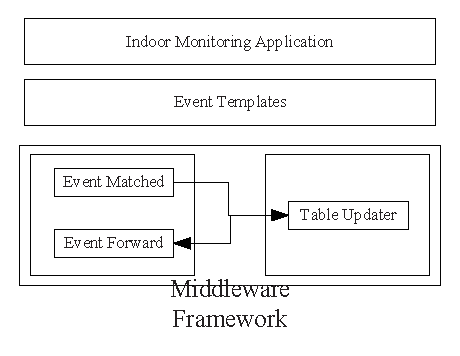
\includegraphics[width=.8\textwidth]{indoor-architecture}
\caption{Architecture of indoor application based on PSWare}
\label{fig:indoor-architecture}
\end{figure}

\subsection{Data Structures}
We used TED for fusion point selection, in this section, we will show what kind of data are maintained by individual sensor nodes so that they will later be used for efficient event detection. We have a set of nodes \(V'\subseteq V\) selected as event fusion points. Each individual sensor nodes will maintain the following table \(table_r\) for all \(v'_n\in V'\)
\begin{itemize}
\item Fusion point ID (\(fid_n\)): the node ID of the fusion point:
\item	Hop count (\(hop_n\)): the number of hops to reach the fusion point
\item	Parent (\(parent_n\)): the next hop to that fusion point\\
\end{itemize}
Each sensor node will also maintain an event table \(table_e\) containing the information for each event type \(e_n\in E\) which includes the following fields:
\begin{itemize}
\item Event type ID (\(e_n\)): the ID which is assigned to each event type
\item Fusion point for the event (\(fusion_n\)): the fusion point at which the event is mostly likely to be detected at the lowest cost.
\item Fusion cost (\(cost_n\)): the fusion cost for event type \(e_n\)\\
\end{itemize}
In addition to the above tables, each fusion point \(v'\in V'\) will maintain another table \(table_m\) for the purpose of matching events. \(table_m\) contains the following fields:
\begin{itemize}
\item Event type ID (\(e_n\)): the ID of the event type
\item Event instance ID (\(i\)): the \(i\)th event instance of event type \(e_n\) (we use \(e_n^i\) to denote such an instance of event)
\item Source node (\(v_n^i\)): the node which forwarded \(e_n^i\) to the fusion point
\item Event timestamp (\(t_n^i\)): the timestamp when the event \(e_n^i\) is detected
\item Detection cost (\(cost_n^i\)): the cost for detecting event \(e_n^i\)
\end{itemize}

\subsection{Table Construction}
Each node \(v_n\) periodically broadcasts messages \(msg_r\) which is its \(table_r\). If the node itself is a fusion point, then it will add itself in \(table_r\) and broadcast the message. The procedure is shown in Procedure \ref{algo:table_r}.

\begin{algorithm}
\begin{algorithmic}
\REQUIRE \(v_n\rightarrow msg_r\)
	\FOR {each entry \(t'\) in \(msg_r\)}
		\IF {\NOT exists \(t'\rightarrow fid_n\) in \(table_r\)}
			\STATE \(addTo(table_r, t')\)
		\ENDIF
		\FOR {each entry \(t\) in \(table_r\)}
			\IF {\(t\rightarrow fid_n = t'\rightarrow f_n\)}
				\IF {\(t'\rightarrow hop_n < t\rightarrow hop_n\)}
					\STATE \(t\rightarrow hop_n \gets t\rightarrow hop_n+1\)
					\STATE \(t\rightarrow parent_n \gets v_n\)
				\ENDIF
			\ENDIF
		\ENDFOR
	\ENDFOR
	\IF {self is fusion point \AND \NOT exists \(self\rightarrow id\) in \(table_r\)}
		\STATE \(addTo(table_r, (self\rightarrow id, 0, self\rightarrow id))\)
	\ENDIF
	\STATE \(msg_r \gets table_r\)
	\STATE \(periodically\_broadcast(msg_r)\)
\end{algorithmic}
\caption{\(table_r\) construction}
\label{algo:table_r}
\end{algorithm}

In addition to \(msg_r\), each \(v'_k\in V'\) will periodically advertise its \(table_m\) by broadcasting \(msg_m\) so that other sensor nodes can construct their \(table_e\) with Procedure \ref{algo:table_e}.

\begin{algorithm}
\begin{algorithmic}
\REQUIRE \(v'_k\rightarrow msg_m\)
	\FOR {each entry \(t'\) in \(msg_m\)}
		\IF {\NOT exists \(t'\rightarrow e_n\) in \(table_e\)}
			\STATE \(addTo(table_e, (t'\rightarrow e_n, 1, v'_k, t'\rightarrow cost_n^i+table_r\rightarrow hop_k))\)
		\ENDIF
		\FOR {each entry \(t\) in \(table_e\)}
			\IF {\(t\rightarrow e_n = t'\rightarrow e_n\)}
				\IF {\(t'\rightarrow cost_n^i+table_r\rightarrow hop_k < t\rightarrow cost_n\)}
					\STATE \(t\rightarrow cost_n \gets t'\rightarrow cost_n^i+table_r\rightarrow hop_k\)
					\STATE \(t\rightarrow fusion_n \gets v'_k\)
				\ENDIF
			\ENDIF
		\ENDFOR
	\ENDFOR
	\IF {self is fusion point}
		\STATE \(msg_m \gets table_m\)
		\STATE \(periodically\_broadcast(msg_m)\)
	\ENDIF
\end{algorithmic}
\caption{\(table_e\) construction}
\label{algo:table_e}
\end{algorithm}

The construction of \(table_m\) will take place when the event instance \(e_n^i\) is detected and forwarded to a fusion point \(v'_n\). We will discuss how forwarding could be done in the next subsection.
\subsection{Event Matching and Forwarding}
When an event \(e_n^i\) is detected at node \(v_k\), node will use \(table_r\) and \(table_e\) to decide how to forward the detected event to the fusion points so that higher level events can be detected. The pseudo code is shown in Procedure \ref{algo:eventforwarding}.

\begin{algorithm}
\begin{algorithmic}
\REQUIRE detected event \(e_n^i\)
	\IF {\(table_e\rightarrow fusion_n=null\)}
		\STATE \(event\_forward(e_n^i)\)
	\ELSE
		\STATE \(send(e_n^i, table_e\rightarrow fusion_n)\)
	\ENDIF
\end{algorithmic}
\caption{Event forwarding}
\label{algo:eventforwarding}
\end{algorithm}

In case the fusion point for event type \(e_n\) has not been decided, the node will forward the event to some of its closet fusion points using the \(event\_forward\) function according to TED. Upon the reception of \(e_n^i\) from \(v_k\), the fusion point will first update its own \(table_m\). Then it will check if there is any composite event \(e_{comp}\) which uses \(e_n\) and another event \(e_j\) as its sub-event (\(e_{comp}=comp(e_n, e_j)\)). The pseudo code of event matching is shown in Procedure \ref{algo:eventmatching}.

\begin{algorithm}
\begin{algorithmic}
\REQUIRE \(e_n^i\) detected by \(v_k\) with cost: \(cost_n^i\)
	\STATE \(addTo(table_m, (e_n, e_n^i, v_k, now(), cost_n^i))\)
	\FOR {each \(e_j\) in \(E\)}
		\IF {\(\exists r\in R\) \AND \(r=e_{comp}=comp(e_n, e_j)\)}
			\FOR {each \(e_j^k\) in \(table_m\)}
				\IF {\(comp(e_n^i, e_j^k)=true\)}
					\STATE \(addTo(table_m, (e_{comp}, e_{comp}^i, self, now(), cost_n^i+cost_j^k))\)
					\STATE \(detected(e_{comp})\)
				\ENDIF
			\ENDFOR
		\ENDIF
	\ENDFOR
	\STATE \(event\_forward(e_n^i)\)
\end{algorithmic}
\caption{Event matching}
\label{algo:eventmatching}
\end{algorithm}

Note that if \(e_{comp}\) has been successfully detected, the procedure will run function \(detected\) which, in turn, will execute Procedure \ref{algo:eventforwarding}. The procedure will also use \(event\_forward\) in the end to forward the detected event to other fusion node so that better fusion point may be found.

\subsection{Event Subscription}
To monitor the temperature change of the entire floor and adjust the air-conditioner accordingly, we need to define a composite event that comprises of the sub-events for individual room. For example, the air conditioner can be adjusted if several adjacent rooms' temperature rises too fast. The primitive and composite event definitions for this purpose are shown in Listing \ref{prog:indoorEvents}.

\begin{lstlisting}[caption=Event definition for temperature monitoring, label=prog:indoorEvents]
Event SingleTemp {
	int id=System.id;
	int temperature=System.temperature;
} where {
	temperature>THRESHOLD
}
Event CompositeTemp {
} on {
	SingleTemp e1, e2, e3;
} where {
	e1.id==1 &&
	e2.id==2 &&
	abs(e1.time - e2.time)<TIME_INTERVAL
}
\end{lstlisting}

The primitive event simply tests if the temperature passes certain threshold while the composite event is the conjunction of several primitive events. We deployed the some Micaz nodes in different rooms in our building as shown in Figure \ref{fig:indoorDeployment}.

For fire alarm, the composite event definition is based on both light and temperature readings. The event definition is shown in Listing \ref{prog:indoorFire}.
\begin{lstlisting}[caption=Event definition for fire alarm, label=prog:indoorFire]
Event Temperature {
	int id=System.id;
	int temperature=System.temperature;
} where {
	temperature>THRESHOLD_TEMP
}
Event Light {
	int id=System.id;
	int light=System.light;
} where {
	light>THRESHOLD_LIGHT
}
Event Fire {
} on {
	Temperature temp;
	Light light;
} where {
	e1.id==light.id
}
\end{lstlisting}
%\section{Application Scenario Two: Intelligent Transportation Systems}
\label{sec:its}
In this section, we use Intelligent Transportation Systems (ITS) as another example application to demonstrate how PSWare can help for application development.

\subsection{Requirement Analysis}
A lot of WSN-based applications can be found in ITS including collision avoidance, traffic light control, automatic road enforcement and electronic toll. Composite event detection is very common in these applications because one of the common requirements for these applications is to detect the speed of vehicle. In this paper, we consider the scenario where the sensor nodes are deployed as road side units (RSU) \cite{klein:its}. Our actual deployment method is illustrated in Figure \ref{fig:itsSensor}.

\begin{figure}
\centering
\subfloat[Road side sensor nodes]{\label{fig:itsSensor1}\figurehalfwidth{itsSensor1.JPG}}
\subfloat[Sensor nodes on the lamp]{\label{fig:itsSensor2}\figurehalfwidth{itsSensor2.JPG}}
\caption{Sensor nodes for transportation systems}
\label{fig:itsSensor}
\end{figure}

Different from the indoor temperature and light monitoring, the ITS applications have the following characteristics:
\begin{itemize}
\item The magnetic sensor used in ITS application will consume much more energy so the energy consumption from sensing may not be negligible.
\item The sensor nodes are deployed and lined up on each road and will detect each passing vehicle one by one.
\item Instead of gathering the data and making a local decision, the vehicles may need to be tracked. 
\end{itemize}
To detect events in such a model, the sensors nodes must not be turned on all the time. Instead, they should be waken up only when an incoming vehicle has been detected by their preceding nodes.

\subsection{Event Forwarding}
The overall system architecture of ITS is similar to the indoor application. However, different from the indoor application, which forward the events according to the link condition and the event detection results, in ITS applications, the events are forwarded along the road. The procedure for nodes' wake-up and forwarding is shown in Procedure \ref{algo:itsForward}. We use the following notations in the procedure:
\begin{itemize}
\item \(V=\{v_1, v_2 \cdots \}\): the sensor nodes that come next on the road. For the sensors on the road, \(\|V\|=1\) but for the sensors next to the crossroads, \(\|V\|>1\)
\item Vehicle events \(e_i\) which are either detected locally or received from another node.
\end{itemize}

\begin{algorithm}
\begin{algorithmic}
	\IF {detected vehicle event \(e_i\)}
		\FORALL {\(v_n\in V\)}
			\STATE forward \(e_i\) to \(v_n\)
		\ENDFOR
	\ENDIF
	\IF {received vehicle event \(e_i\) from \(v_m\)}
		\STATE start data collection
		\IF {detected vehicle event \(e_j\)}
			\STATE select \(e_i\) and \(e_j\) for composite event detection
		\ELSE
			\STATE wait for event to expire
		\ENDIF
		\STATE stop data collection
	\ENDIF
\end{algorithmic}
\caption{Event forwarding for ITS}
\label{algo:itsForward}
\end{algorithm}

In the actual application deployment, we use some sentry nodes at the entrances of the deployed area. These nodes have more power and will monitor the entrance for newly entered cars. Except for the sentry node, the nodes will not actively collect data until it receives messages from others. Once the event from the previous node on the road is received, it will be selected for composite event detection.

\subsection{Event Subscription}
As one of the most basic events used by many ITS applications, we show the event definitions for tracking the vehicles in Listing \ref{prog:carEvent}.

\begin{lstlisting}[caption=Event definition for tracking vehicles, label=prog:carEvent]
Event CarEvent {
	int time=System.time;
	int magnetic=System.magnetic;
	int location=System.location;
} where {
	magnetic>THRESHOLD
}
Event SpeedEvent {
	int speed=(e1.location-e2.location)/(e1.time-e2.time);
} on {
	CarEvent e1, e2;
} where {
	e1.time>e2.time &&
	speed>THRESHOLD
}
\end{lstlisting}

First, an event named 'CarEvent' is defined to detect the presence of the individual vehicles. Then based on this event, we can have a composite event to measure the speed of the car.
%\section{Application Scenario Three: Intelligent Car Park}
The final application that we are going to show in this paper is an intelligent car park \cite{tang:carpark}. It is related to ITS but there are a few distinct features with it so we will talk about it in a separate section.

\subsection{Requirement Analysis}
An intelligent car park application is different from other ITS applications in the following ways:
\begin{itemize}
\item Vehicle tracking is usually not needed. The application user is probably more interested in how many parking spaces have been occupied and how many are still available.
\item The sensor nodes probably shouldn't be deployed on the road. Instead, they should be deployed on each parking space to monitor its availability.
\item Different from other ITS applications, the message delay in intelligent car park is not really important. Message delay for a couple of seconds is probably acceptable. However, each message must be reliably delivered.
\item The environment for message transmission may be harsh and message lost may be common.
\end{itemize}

\begin{figure}
\centering
\subfloat[The sensor node]{\label{fig:carParkSensor1}\figurehalfwidth{carParkSensor1.JPG}}
\subfloat[The light sensor]{\label{fig:carParkSensor2}\figurehalfwidth{carParkSensor2.JPG}}
\caption{Car park sensor platform}
\label{fig:carParkSensor}
\end{figure}

\subsection{System Deployment}
We used the campus car park as our test bed. We deployed some micaz sensor nodes for the application. For simplicity, we use light sensor to detect the presence of a vehicle. For better communication, the sensor nodes are attached close to the ceiling instead of on the ground. The light sensor on each node is connected through an extended cable as shown in Figure \ref{fig:carParkSensor}. 

\begin{figure}
\centering
\figurecurrentwidth{carParkDeployment}
\caption{Car park sensor deployment}
\label{fig:carParkDeployment}
\end{figure}

The deployment of the individual sensor nodes is shown in Figure \ref{fig:carParkDeployment}. In such a system, the management is interested in the number of park spaces and the location of them \cite{tang:carpark}. Therefore, each parking space is monitored by one sensor node.

\subsection{Event Subscription}
The primitive events for such a system will be the availability of individual car park spaces. Based on the primitive event, if we want to get notified when the parking spaces near the exit become available, then we just need to define composite events which locate the spaces with certain IDs. Th event definitions are shown in Listing \ref{prog:carPark}. Here, the composite event takes two primitive events for parking space \(1\) and \(2\) which are close to the exit.

\begin{lstlisting}[caption=Event definition for a car park, label=prog:carPark]
Event ParkSpaceEvent {
	int id=System.id;
	int time=System.time;
	int light=System.light;
} where {
	light>THRESHOLD
}
Event CarParkEvent {
	int id=System.id;
} on {
	ParkSpaceEvent e1, e2;
} where {
	e1.id==1 ||
	e2.id==2 ||
	e1.time-e2.time<10
}\end{lstlisting}
\section{Evaluation}
\label{sec:experiments}
In this section, we evaluate PSWare. We first introduce the metrics we use for performance evaluation. Then, we present the evaluation results based on the three application cases discussed in the previous section. 

\subsection{Performance Metrics}
The primary of PSWare is help developing WSN-based applications. However, additional overhead may be introduced by its event detection framework. Therefore, we use the following metrics to evaluate PSWare:
\begin{itemize}
\item Memory usage: since the sensor nodes have limited amount of memory, it is important to know the memory overhead introduced by PSWare in order to evaluate its practical use. 
\item Message cost: it is useful to measure the application message cost when using customized event processing mechanism. This way, we can show how PSWare is helpful in deploying real applications. The message cost is obtained by setting up a counter inside the sensor node. The counter will be written into flash so that we can retrieve it after the experiments.
\item Event detection delay: some event processing mechanisms aims at shortening the event detection delay. In this paper, we measure the time between the subscription is disseminated and the event is notified.
\end{itemize}

For each of the application case discussed in the previous section, we implemented an additional opportunistic event detection mechanism where all the events are transmitted to the sink for detection. The transmission is done using the existing routing protocol, CTP, provided by TinyOS. This serves as reference when studying the performance.

\subsection{Results}
In the car park application, the messages indicating the occupancy of the cars must be reliably delivered to the control center. Therefore, we implemented a retransmission mechanism for event delivery. With PSware, the application takes 61k bytes of code and 1.5k bytes of data. Without PSWare, the application takes around 35k bytes for code and 1.3k bytes for data. For the evaluation, we primarily consider only the message costs because the delay isn't that important in such a system. The experimental results for the car park are shown in Figure \ref{fig:carParkResults}. The message cost is highest during rush hour when there are a lot of cars entering and leaving the car park. To further study application under different settings, we used two deployment strategies. The first one is even deployment, where all the parking spaces in a particular area are deployed. In the second strategy, we assume the management is only interested in a subset of the parking spaces so we randomly deployed the sensor nodes in some of the parking spaces. For all the experiments as we can see, the message cost by using application-specific middleware for ITS is the lowest while the opportunistic way is the highest.

\begin{figure}
\centering
\subfloat[With random fusion point deployment]{\label{fig:carParkResult1}\figurehalfwidth{carParkResult1}}
%\qquad
\subfloat[With even fusion point deployment]{\label{fig:carParkResult2}\figurehalfwidth{carParkResult2}}
\caption{Car park experiment results}
\label{fig:carParkResults}
\end{figure}

The next application we evaluate is ITS. One distinct feature of ITS is that we can make use of the special road deployment of the sensor nodes to make event processing easier. As a result, by replacing the default event processing algorithm with a simpler one that processes the event along the road, both code and data sizes are reduced. Without PSWare, the application takes around 25k bytes for code and 1.2k bytes for data. With PSware, it takes around 51k bytes of code and 1.4k bytes of data. The results for ITS are shown in Figure \ref{fig:itsResults}. Different from the car park application, such applications are more delay sensitive. So we also measured the time delay for the event detection. %Similar to the car park application, ITS-specific event detection mechanism can save most energy. Both ITS and TED will introduce certain amount of delay due to the waiting.
 
\begin{figure}
\centering
\subfloat[Message cost]{\label{fig:itsResult1}\figurehalfwidth{itsResult1}}
%\qquad
\subfloat[Delay]{\label{fig:itsResult2}\figurehalfwidth{itsResult2}}
\caption{Experiments on the roads}
\label{fig:itsResults}
\end{figure}

Our final experiments is for the indoor monitoring application. We consider the application scenario where the sensor nodes are deployed in a building so that the temperature can be monitored. With PSware, the application takes 58k bytes of code and 1.5k bytes of data. Without PSWare, the application takes around 34k bytes for code and 1.3k bytes for data. The application As discussed in the previous sections, such an application can probably be useful for certain types of context aware pervasive applications such as indoor temperature monitoring. The experimental results is shown in Figure \ref{fig:itsResults}. 

\begin{figure}
\centering
\subfloat[With random fusion point deployment]{\label{fig:indoorResult1}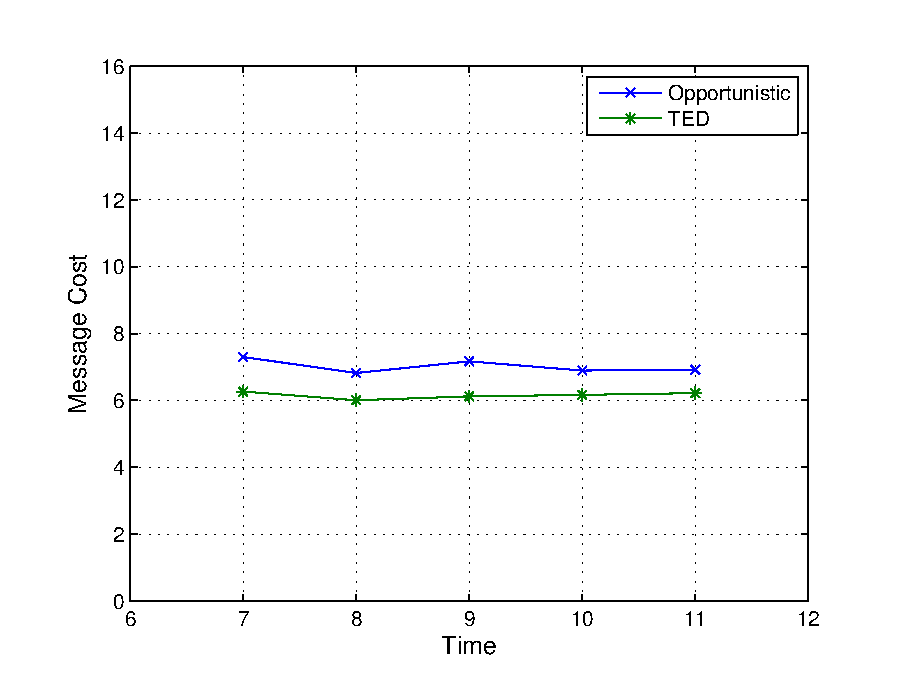
\includegraphics[width=.5\textwidth]{indoorResult1}}
%\qquad
\subfloat[With even fusion point deployment]{\label{fig:indoorResult2}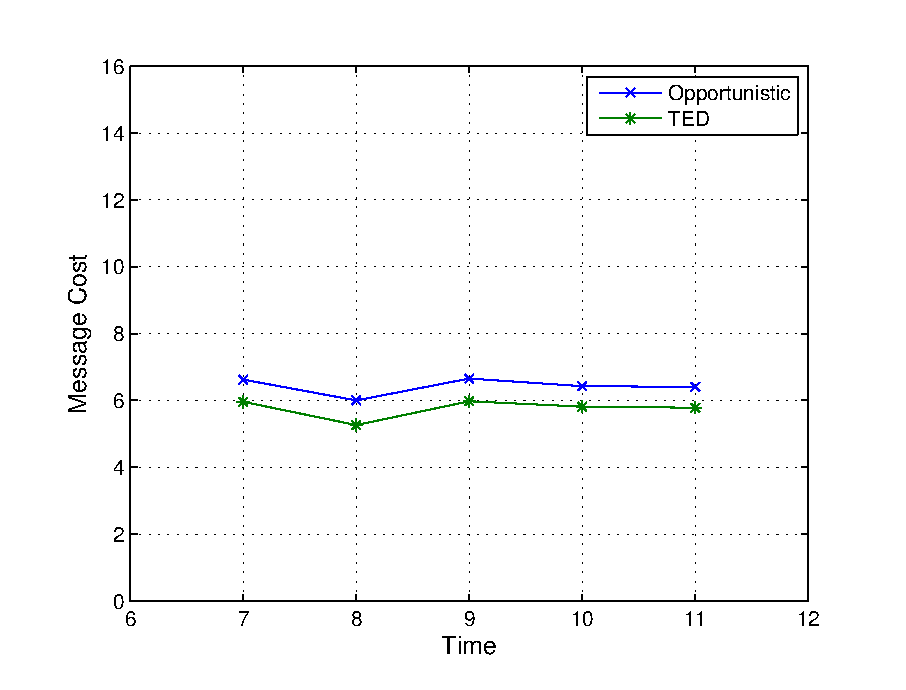
\includegraphics[width=.5\textwidth]{indoorResult2}}
\caption{Experiments for temperature monitoring}
\label{fig:indoorResult}
\end{figure}

\section{Conclusion}
\label{sec:conclusion}
In this paper, we presented PSWare, a flexible middleware framework for composite events processing. PSWare uses a flexible architecture where different event detection mechanisms may easily integrated. We described the design of PSWare and explained how it can be customized for different applications. Then we gave two examples of using PSWare. The first one implements a more general composite event algorithm while the second one uses an application-specific event detection approach. Based on our implementation, we performed experiments and demonstrate the effectiveness of PSWare for prototyping and performance comparison.

\bibliographystyle{plain}
\bibliography{../references/wsn-general,../references/wsn-aggregation,../references/wsn-middleware,../references/wsn-pubsub,../references/edl,../references/pubsub,../references/algorithms,../references/event-detection,../references/pervasive,../references/shm}
\end{document}